\scanpage{37}
\mspage{18}
\margin{le passage de $u$ \unsure{à|:} $\tau(u)$ s'exprime par
\[
\begin{aligned}
\lambda&\longmapsto\varepsilon_0^{-1}(\tau_\infty(\lambda^{-1}))\\
(\lambda&\longmapsto\lambda\quad\text{si }\lambda=l_0^\gamma)\\
\eta&\longmapsto\tau_\infty(\eta)\\
\xi&\longmapsto\widetilde\sigma_\infty(\xi)=\sigma_\infty\tau_\infty(\xi)
\end{aligned}
\]}
\[
(63)\qquad
\begin{array}{||l||}
\left\{\begin{aligned}
\beta'&=\alpha'\sigma_\infty(\lambda)\quad(=\alpha'l_1^\gamma\text{ si }\lambda=l_0^\gamma)\\
\text{avec}\qquad\alpha'&=\xi'\rho^{\unsure{\deleted{-1}|-1}}(\xi')^{-1}\\
\beta'&=\eta\sigma_\infty\unsure{(\eta)|\eta)}^{-1}
\end{aligned}\right.\\\hline\hline
\end{array}
\]
\margin{\uline{NB} L'ens. des relations stable par substitutions de la forme
\[
\begin{aligned}
\xi'&\longmapsto l_0^H\xi\\
\eta&\longmapsto l_0^H\eta\\
\text{i.e}\quad\alpha'&\longmapsto l_0^{\unsure{H|\mu}}\alpha'l_1^{-\unsure{H|\mu}}\\
\beta'&\longmapsto l_0^{\unsure{H|\mu}}\beta'l_1^{-\unsure{H|\mu}}
\end{aligned}
\]}
Ici, les quantités $\alpha',\beta',\xi'$ ont été introduites en termes des quantités primitives
$\lambda,\eta,\xi$ $(\longmapsto\beta,\deleted{\unsure{\alpha}}\alpha,\widetilde\alpha)$,
s'introduisant ds les formules (54) (et (57)), par le pur calcul \deleted{\unsure{en}} \inserted{ds}
$\widehat\Pi_{03}$, comme donnant lieu aux formules les plus \unsure{symétriques|sympathiques}.
Mais on peut les interpréter aussi de façon ``géométrique'', en posant
(\deleted{\unsure{avant}} \inserted{pour} ce qui est de $\beta',\deleted{\unsure{\beta}}\inserted{\alpha'},\widetilde\alpha'$)
\[
(64)\qquad
\begin{aligned}
b_i^{\prime\omega}&=(b_i^\omega)^{-1},\qquad&
\unsure{(|\deleted{(}}\widetilde b_i^{\prime\omega}&=(\widetilde b_i^\omega)^{-1},\qquad&
\widetilde a_i^{\prime\omega}&=(\widetilde a_i^\omega)^{-1}\\
&=b_i^{\omega'}&&&&
\end{aligned}
\]
de sorte que les formules (57) deviennent
\[
(65)\qquad\left\{\begin{aligned}
u(b_i^{\prime\omega})&=\varphi_{\omega i}^\omega(\beta')b_i^{\prime\omega}\\
u(\widetilde b_i^{\prime\omega})&=\varphi_{\omega i}^\omega(\alpha')\widetilde b_i^{\prime\omega}\\
u(\widetilde a_i^{\prime\omega})&=\widetilde a_i^{\prime\omega}\psi_{\omega i}^\omega(\widetilde\alpha')
\end{aligned}\right.
\]
Enfin, la quantité $\xi'=\eta\xi$ est obtenue géométriquement, en introduisant les chemins
\diagram{
$(66)\qquad$
\begin{tikzcd}[ampersand replacement=\&,column sep=large,row sep=large]
\widetilde d_i^{\prime\omega}:\&P^\omega\arrow[rr]\arrow[dr,"d_{\omega i}^\omega"']\&\&R_i^{\omega'}\\
\&\&Q_{\omega i}\arrow[ur,"c_{\omega i}^\omega"']\&
\end{tikzcd}
\qquad$\widetilde d_i^{\prime\omega}=c_{\omega i}^\omega\cdot d_{\omega i}^\omega$
}
\figure{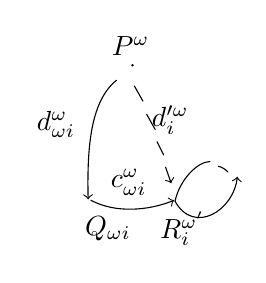
\begin{tikzpicture}[x=.012cm,y=-.012cm,line cap=round,line join=round]
\fill (128,72) circle[radius=1.4];
\draw[->] (111,88)..controls (82,111) and (80,165)..(81,214);
\draw (130,94)--(139,110);
\draw (143,124)--(152,140);
\draw (154,153)--(161,167);
\draw[->] (163,180)--(169,197);
\draw[->] (84,215)..controls (110,229) and (145,226)..(172,215);
\draw[->] (173,216)..controls (193,252) and (235,226)..(239,190);
\draw (173,216)..controls (178,193) and (197,174)..(210,174);
\draw (219,179)..controls (223,180) and (226,182)..(229,185);
\node at (126,52) {$P^\omega$};
\node at (47,135) {$d_{\omega i}^\omega$};
\node at (168,130) {$d_i^{\prime\omega}$};
\node at (124,196) {$c_{\omega i}^\omega$};
\node at (102,245) {$Q_{\omega i}$};
\node at (181,245) {$R_i^{\omega'}$};
\end{tikzpicture}}
par la formule
\margin{36}
